\documentclass[../r.tex]{subfiles}

\begin{document}

\section{Volunteering Experience}
Besides the Perfect Environs project:
\begin{enumerate}
\item I created problems for SwampCTF.
\item I modernized a blacksmithing website.
\item I helped build stands for GWIZ Science Museum.
\item I created an exhibit for TEDx Sarasota.
\end{enumerate}
\subsection{Perfect Environs}
Created a GIS native plant mapping tool for Florida native plant experts using Google Maps/FT, JS, KML, LAMP.
\begin{enumerate}
\item Found the data on an archive site. 
\item Converted it to the appropriate format to upload to Maps/FT
\item Linked the plant associations and climate regions to custom native plant pages populated with a MySQL database.
\item Created these pages in a landscaping focused format, connecting them to wikipedia and plant image/nursery sites (FANN/FNPS).
\item Created drawing tools for adding microhabitats of arbitrary multigon complexity. 
\item Added mediawiki and forum with FluxBB.
\end{enumerate}

I worked on this with a native plant expert who has recently passed away.  Here's a photo of him with the application we built together.  We unveiled the website that hosted an interactive version of \href{https://www.plantrealflorida.org/images/maps/vegetation_map_large.pdf}{this map} at a conference in Plant City in 2013. It was the keynote speech. I still remembered how the audience continued audibly gasping as he introduced the new features that I had developed.

\href{http://perfectenvirons.com/About_The_Designer.html}{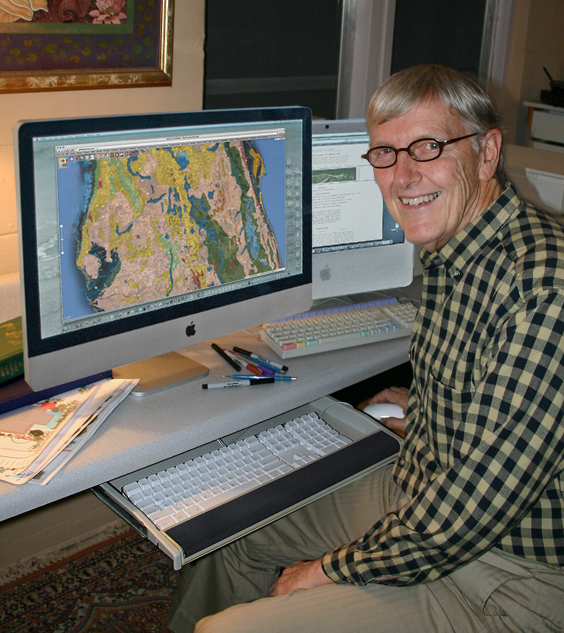
\includegraphics[scale=0.3]{../fun/Michael_Clendenin_Miller564x633.jpg}}

%\subsection{Florida Blacksmithing}



\end{document}